\begin{table*}
  \centering
  \begin{tabular}{cc}
    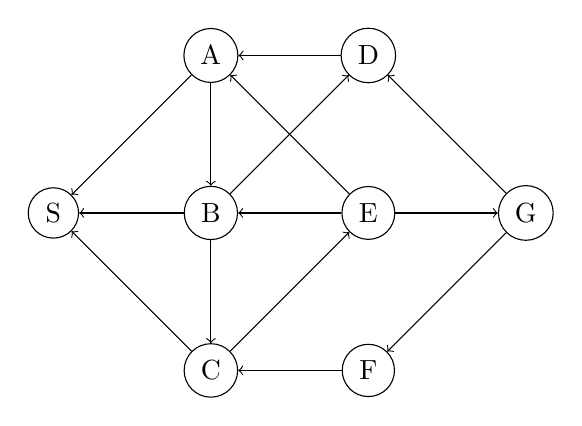
\begin{tikzpicture}[->, auto, node distance=2cm, every node/.style={circle, draw, minimum size=.5cm}]
      \node (S) {S};
      \node (B) [right of=S] {B};
      \node (A) [above of=B] {A};
      \node (C) [below of=B] {C};
      \node (D) [right of=A] {D};
      \node (E) [below of=D] {E};
      \node (F) [below of=E] {F};
      \node (G) [right of=E] {G};

      \path[every node]
      (A) edge (S) edge (B)
      (B) edge (S) edge (C) edge (D)
      (C) edge (S) edge (E)
      (D) edge (A)
      (E) edge (A) edge (B) edge (G)
      (F) edge (C)
      (G) edge (D) edge (F)
      ;
    \end{tikzpicture} &

    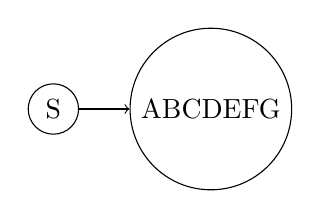
\begin{tikzpicture}[->, auto, node distance=2cm, every node/.style={circle, draw, minimum size=.5cm}]
      \node (S) {S};
      \node (ABCDEFG) [right of=S] {ABCDEFG};

      \path[every node]
      (S) edge (ABCDEFG);
    \end{tikzpicture}                     \\
    transponierter Graph                                                             & Komponentengraph
  \end{tabular}
\end{table*}